%\include{appendix}


\documentclass[doublespaced, 12pt]{article}
\usepackage{natbib}
\usepackage{pdfpages}
\usepackage{float}
\usepackage{graphicx}
\graphicspath{{F:/study/university life/BIOINFO/bcb420/Code/Systemikon/STAT/pictures/}}

%\usepackage[framed,numbered,autolinebreaks,useliterate]{mcode}

\title{STATS Documentation}
\author{Rui Xu}

\begin{document}

\maketitle

\begin{abstract}
This documentation is about the STATS section in the Systemikon workbench. This section contains various statistic manipulation tool and some systematic biology analysis for systematic interpretation and downstream work. 
\end{abstract}

\section{Introduction}
Due to the increasing number of biological databases with different but related datatypes, analysis of several data types at same time can be used to generate more reliable prediction. However, the statistical analysis and manipulation must be applied before trying to interpret systematic functions and significance. In the project, two kinds of upstream outputs are generated from upstream, graphic output and numerical output, the graphic output including a defined network with numbers of systems(clusters) and numerical output is just the numerical version of the network including the nodes interaction(edge lists) and their weights. 

\section{Code Description}
\subsection{Code overview}
The following requires the R,Python and several R packages. A functional R server is required to generate output. The code may be changed if the upstream format is changed

\subsection{Code Functions}
\begin{itemize}
	\item Numerical Permutation \\ This Code randomly first choose GeneID and system ID of the upstream output and extract them from original output, then randomly assigns genes into different system and rewrite them back into original data frame. 2 outputs are generated from the code, first one is the output including permuted data and second one is system size data used for power law analysis. 
	\item Graph Permutation \\ This code is used to randomized multi graph.The program will swap two edges while preserving their degree distribution,for some reason rewire function in igraph package doesn't work on imported graph and it can not rewire weights of the edges, so my own version of graphic randomization is coded based on networkx package from Python. They worked in same way and basic principle is outlined in the article under the folder 
	\item Perturbation \\This code generally introduce perturbations into the system so that robustness can be tested in the future, the code consists two part, first part of the code introduce little noise to the track scores obtained from upstream, it will either add or subtract a small number to the original score(the range of the noise is a parameter of input). Second part of the code can be used to remove a portion of the original data, for example, the ranked system sizes can be analysed by this manipulation,portion of the size data can be discarded and run powerlaw analysis again to test robustness.
	\item Powerlaw analysis \\ This code function to analysis the size distribution of the network. Many biological features follow the pattern of power law distribution,Where one quantity varies as a power of the other.The code first counts many nodes are contained in different system(cluster) and rank them in decreasing order. Then R package PoweRlaw is used to obtain power law analysis of such input. The output will be a plot where x-axis represents rank of system size and y-axis represents the degree of each system(largest size will have a degree of one). In the plot,there will be two fitted lines, red line is the fitted log normal and green line is fitted Powerlaw.
	\item Betweenness of the network \\ Centralities are important in biological network, the node with low Eigenvector centrality but high Betweenness centrality may have more influence to other nodes while the node with high Eigenvector centrality but low Betweenness centrality has direct contact to important node. In this part, the code is designed to plot Eigenvector centrality against Betweenness centrality and find point of interest and visualize them in the original network.
\end{itemize}




\section{Input and Output}
\subsection{Numerical Permutation}
\textbf{Input}: Numerical Permutation is obtained from upstream in 8 columns:Gene 1   Gene2   TrackScore 1  TrackScore 2  TrackScore 3  TrackScore 4  System for Ge2  System for Ge2\\
\textbf{Operation}:Code will reassign genes into random system and plug back into the original chart\\
\textbf{Output}:output example is provided in the \underline{numerical permutation} folder

\subsection{Graph Permutation}
\textbf{Input}:the input files has to follow this specific 3 columns format: Node 1   Node 2   Weight.\\
\textbf{Operation}:Code will swap the edges from input edgelist and randomize the multigraph.\\
\textbf{Output}:output example is provided in the \underline{graphic permutation} folder

\subsection{Perturbation}
\textbf{Input}:The input file has the same format with input file of Numerical Permutation\\
\textbf{Operation}:Code will introduce noise and take out certain portion of the input data\\
\textbf{Output}:output example is provided in the \underline{perturbation} folder

\subsection{Powerlaw analysisn}
\textbf{Input}:The input file is list of numbers which represents which system does each gene belong to.\\
\textbf{Operation}:Code will analyse size distribution and make fitted lines on the plot \\
\textbf{Output}:output example is provided in the \underline{Powerlaw} folder and here is an example picture 
\begin{center}
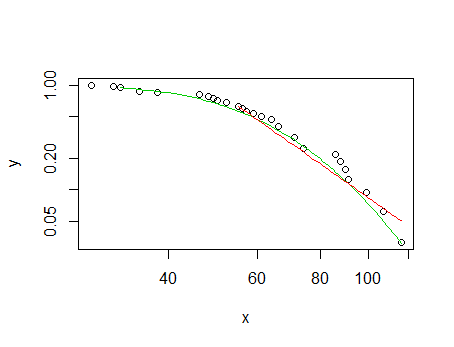
\includegraphics[scale=0.8]{powerlaw}
\end{center}

\subsection{Betweenness of the network}
\subsection{Powerlaw analysisn}
\textbf{Input}:The input file has the same format as Graphic Permutation\\
\textbf{Operation}:Code will calculate Eigenvector centrality and Betweenness centrality,then plot them against each other.Code also can be used to label point of interest in the network \\
\textbf{Output}:output example is provided in the \underline{Betweenness analysis} folder and here is an example picture 
\begin{center}
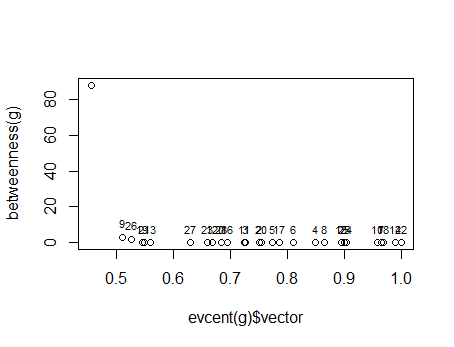
\includegraphics[scale=0.8]{outputscatterplot}
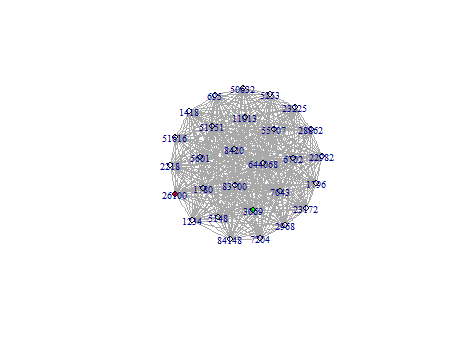
\includegraphics[scale=0.8]{outputimage}
\end{center}

\section{Conclusion}
More statistic analysis will be included in the future, for example, Silhouette Plot function need to calculate clusters first,so it is necessary to get access to other faster computers.Furthermore,Algorithms for some of the code can be improved, I can foresee that my multigraph permutation code will run very slow when dealing with large amount of data. 

\end{document}